\documentclass[letterpaper,12pt]{article}

\usepackage{threeparttable}
\usepackage{geometry}
\geometry{letterpaper,tmargin=1in,bmargin=1in,lmargin=1.25in,rmargin=1.25in}
\usepackage[format=hang,font=normalsize,labelfont=bf]{caption}
\usepackage{amsmath}
\usepackage{multirow}
\usepackage{array}
\usepackage{delarray}
\usepackage{amssymb}
\usepackage{amsthm}
\usepackage{lscape}
\usepackage{natbib}
\usepackage{setspace}
\usepackage{float,color}
\usepackage[pdftex]{graphicx}
\usepackage{pdfsync}
\usepackage{verbatim}
\usepackage{placeins}
\usepackage{geometry}
\usepackage{pdflscape}
\synctex=1
\usepackage{hyperref}
\hypersetup{colorlinks,linkcolor=red,urlcolor=blue,citecolor=red}
\usepackage{bm}


\theoremstyle{definition}
\newtheorem{theorem}{Theorem}
\newtheorem{acknowledgement}[theorem]{Acknowledgement}
\newtheorem{algorithm}[theorem]{Algorithm}
\newtheorem{axiom}[theorem]{Axiom}
\newtheorem{case}[theorem]{Case}
\newtheorem{claim}[theorem]{Claim}
\newtheorem{conclusion}[theorem]{Conclusion}
\newtheorem{condition}[theorem]{Condition}
\newtheorem{conjecture}[theorem]{Conjecture}
\newtheorem{corollary}[theorem]{Corollary}
\newtheorem{criterion}[theorem]{Criterion}
\newtheorem{definition}{Definition} % Number definitions on their own
\newtheorem{derivation}{Derivation} % Number derivations on their own
\newtheorem{example}[theorem]{Example}
\newtheorem{exercise}[theorem]{Exercise}
\newtheorem{lemma}[theorem]{Lemma}
\newtheorem{notation}[theorem]{Notation}
\newtheorem{problem}[theorem]{Problem}
\newtheorem{proposition}{Proposition} % Number propositions on their own
\newtheorem{remark}[theorem]{Remark}
\newtheorem{solution}[theorem]{Solution}
\newtheorem{summary}[theorem]{Summary}
\bibliographystyle{aer}
\newcommand\ve{\varepsilon}
\renewcommand\theenumi{\roman{enumi}}
\newcommand\norm[1]{\left\lVert#1\right\rVert}

\begin{document}

\begin{titlepage}
\title{Title of My Paper \thanks{You can put thanks here, affiliation here, anything you want here.}
       }
       \author{
  Your Name\footnote{Your University, Your Department, Academic address, (???) ???-????, \href{mailto:your.emailr@uchicago.edu}{your.emailr@uchicago.edu}.} \\[-2pt]
  \and
  Other Name\footnote{Your University, Your Department, Academic address, (???) ???-????, \href{mailto:your.emailr@uchicago.edu}{your.emailr@uchicago.edu}.}}
\date{March 2018 \\
  \scriptsize{(version 18.03.a)}}
\maketitle
\vspace{-9mm}
\begin{abstract}
\small{Put abstract here.
\vspace{3mm}

\noindent\textit{keywords:}\: Static scoring, revenue estimates, dynamic scoring.

\vspace{3mm}

\noindent\textit{JEL classification:} D91, E21, H30
}

\end{abstract}
\thispagestyle{empty}
\end{titlepage}


\begin{spacing}{1.5}{}

\section{Introduction}\label{SecIntro}

  Put introduction here. You'll probably want some references here like \citet{Auerbach:1996} or \citet{DEPR2015}. These citations use the \texttt{natbib} package above and require a call to the \texttt{bibliography} command just before the appendix section.


\section{Model}\label{SecModel}

  Put model description here.


\section{Data}\label{SecData}

  Put data description here.


\section{Estimation}\label{SecEstimation}

  Put estimation details here. You might want to use a table. Table \ref{TabTable1} is an example of a table generated by the code below.

  \begin{table}[htbp] \centering \captionsetup{width=5.8in}
    \caption{\label{TabTable1}\textbf{Percent change in macroeconomic variables over the budget window and in steady-state from policy change}}
      \begin{threeparttable}
      \begin{tabular}{>{\scriptsize}l |>{\scriptsize}r >{\scriptsize}r >{\scriptsize}r >{\scriptsize}r >{\scriptsize}r >{\scriptsize}r >{\scriptsize}r >{\scriptsize}r >{\scriptsize}r >{\scriptsize}r |>{\scriptsize}r >{\scriptsize}r}
      \hline\hline
      \multicolumn{1}{c}{\scriptsize{Macroeconomic}} & & & & & & & & & & & \multicolumn{1}{c}{\scriptsize{2016-}} & \\[-2mm]
      \multicolumn{1}{c}{\scriptsize{variables}} & 2016  & 2017  & 2018  & 2019  & 2020  & 2021  & 2022  & 2023  & 2024  & 2025 & \multicolumn{1}{c}{\scriptsize{2025}} & \multicolumn{1}{c}{\scriptsize{SS}} \\
      \hline
      GDP & 0.54  & 0.50  & 0.55  & 0.91  & 0.90  & 1.02  & 1.03  & 1.02  & 1.03  & 1.22  & 0.87  & 1.40 \\
      Consumption & 0.21  & 0.28  & 0.35  & 0.44  & 0.52  & 0.58  & 0.65  & 0.70  & 0.75  & 0.86  & 0.53  & 1.30 \\
      Investment & 1.28  & 0.99  & 0.98  & 1.93  & 1.74  & 1.96  & 1.88  & 1.72  & 1.67  & 2.02  & 1.62  & 1.65 \\
      Hours Worked & 0.83  & 0.71  & 0.73  & 1.25  & 1.16  & 1.27  & 1.23  & 1.15  & 1.13  & 1.37  & 1.08  & 1.27 \\
      \hline
      Avg. Wage & -0.29 & -0.21 & -0.19 & -0.35 & -0.26 & -0.26 & -0.20 & -0.13 & -0.09 & -0.15 & -0.21 & 0.13 \\
      Interest Rate & 1.00  & 0.72  & 0.66  & 1.20  & 0.90  & 0.91  & 0.70  & 0.47  & 0.33  & 0.56 & 0.75  & -0.51 \\
      \hline
      Total Taxes & -3.59 & -2.42 & -3.10 & -8.23 & -8.21 & -8.36 & -8.32 & -8.53 & -8.89 & -8.27 & -6.71 & -7.43 \\
      \hline\hline
    \end{tabular}
    % \begin{tablenotes}
    %   \scriptsize{\item[]Note: Maybe put sources here.}
    % \end{tablenotes}
    \end{threeparttable}
  \end{table}


\section{Experiment}\label{SecExperiment}

  Put experiment results here. You might want to include a figure. Here is a some figure code that generated Figure \ref{FigLogAbility}. Note that I put my images in an \texttt{images} folder in the directory of this \LaTeX file.

  \begin{figure}[htb]\centering \captionsetup{width=4.0in}
    \caption{\label{FigLogAbility}\textbf{Exogenous life cycle income ability paths $\log(e_{j,s})$ with $S=80$ and $J=7$}}
    \fbox{\resizebox{4.0in}{2.7in}{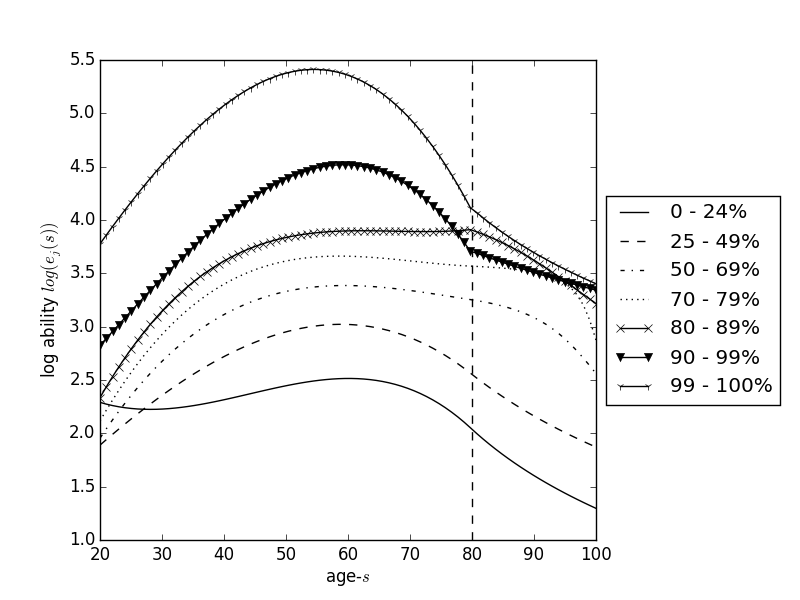
\includegraphics{./images/ability_log_2D.png}}}
  \end{figure}


\section{Conclusion}\label{SecConclusion}

  Put conclusion here.

  \clearpage


\end{spacing}


\newpage
\bibliography{LaTeX_projtemplate.bib}


\newpage
\renewcommand{\theequation}{A.\arabic{section}.\arabic{equation}}
                                                 % redefine the command that creates the section number
\renewcommand{\thesection}{A-\arabic{section}}   % redefine the command that creates the equation number
\setcounter{equation}{0}                         % reset counter
\setcounter{section}{0}                          % reset section number
\section*{APPENDIX}                              % use *-form to suppress numbering

\begin{spacing}{1.0}

\section{Some Appendix}\label{AppSomeAppendix}

  You can put appendices here at the end of the paper using section commands.




\end{spacing}

\end{document}
